\documentclass[10pt,a4paper]{article}
\usepackage[margin=2.2cm]{geometry}
\usepackage{fontspec}
\usepackage{kotex}
\setmainfont{Apple SD Gothic Neo}
\setsansfont{Apple SD Gothic Neo}
\usepackage{amsmath,amssymb}
\usepackage{graphicx}
\usepackage{booktabs}
\usepackage{caption}
\usepackage[dvipsnames]{xcolor}
\usepackage[colorlinks=true,linkcolor=MidnightBlue,citecolor=MidnightBlue,
            urlcolor=MidnightBlue]{hyperref}
\usepackage{titlesec}
\titleformat{\section}{\large\bfseries}{\thesection}{0.6em}{}
\titleformat{\subsection}{\normalsize\bfseries}{\thesubsection}{0.5em}{}
\captionsetup{font=small,labelfont=bf}
\setlength{\parskip}{0.35em}
\setlength{\parindent}{0pt}

\usepackage{mdframed}
\newmdenv[linewidth=0.4pt,linecolor=gray!60,backgroundcolor=gray!5,
          innertopmargin=6pt,innerbottommargin=6pt,skipabove=8pt,skipbelow=8pt]{claimbox}
\newcommand{\claim}[2]{\begin{claimbox}\textbf{주장.} #1\par\smallskip
  \textcolor{gray!70}{\textbf{반증 조건.} #2}\end{claimbox}}

\title{\bfseries 열 둘을 뺐더니 사십 퍼센트가 붙었다\\[2pt]
\large 그리고 $0.0002$ 앞에서 멈췄다}
\author{월드모델 실험실 · 노트 $787 \sim 788$}
\date{2026-08-07}
\begin{document}\maketitle

\section{한 줄}

논문 $156$ 은 만화 세 열을 집 밖으로 옮겨 KR $\Delta +0.0177$ 을 얻고 서랍에 넣으면서
\textbf{다시 꺼낼 조건 ②}를 값으로 적었다 --- \emph{``어느 열이 냈나를 갈라 한 열이 신호의
$2/3$($0.0154$) 이상이면 $1$열로 다시 잰다.''}

\textbf{그 조건이 발동했다.} \texttt{mg\_nauthor}(작가 수 · $9$값) 혼자가
$\mathbf{+0.0239}$ 를 내고, 뽑기 $6$ 으로 굳히니 $\mathbf{+0.0272}$ 다 ---
\textbf{세 열 묶음($0.0231$)보다 크다.}

집 밖으로 $1$열만 옮기니 KR $\Delta$ 가 $0.0177 \to \mathbf{0.0248}$ 로
\textbf{$40\%$ 올랐고 전이율이 $76.6\% \to 91.3\%$ 로 올랐다.}

\textbf{그리고 문턱 $0.025$ 에 $\mathbf{0.0002}$ 모자라 미달이다.} 사전등록한 문턱을
결과 보고 바꾸지 않는다.

\begin{figure}[t]\centering
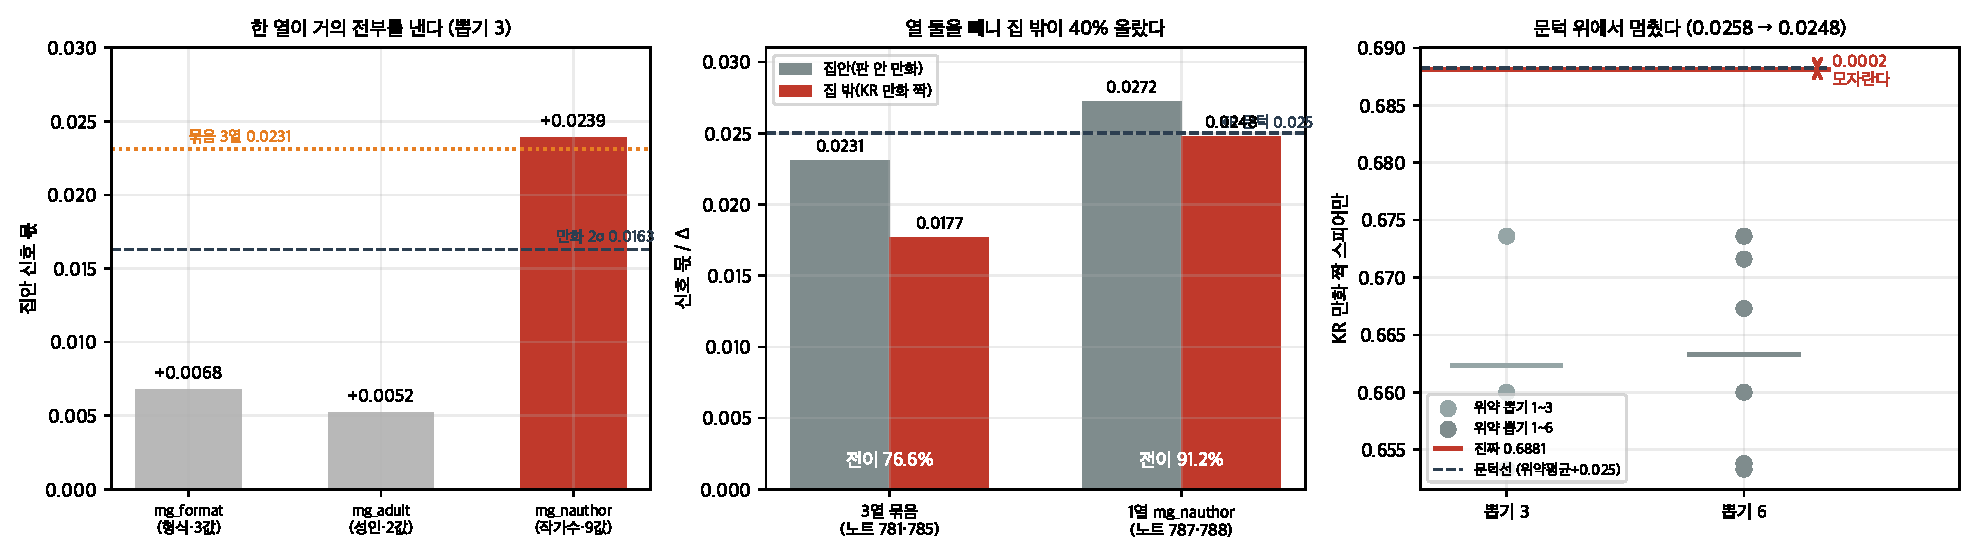
\includegraphics[width=0.99\textwidth]{figs/onecol.pdf}
\caption{왼쪽: \textbf{한 열이 거의 전부를 낸다.} 가운데: \textbf{열 둘을 빼니 집 밖이
$40\%$ 올랐다} --- 막대 안 숫자는 전이율. 오른쪽: \textbf{$0.0002$ 앞에서 멈췄다.}}
\end{figure}

\section{어느 열이 냈나 --- 갈라 봤다}

\textbf{뽑기 $3$ 은 고르기에만 쓴다}(규약 $38$). 열 하나씩 넣고 위약 $3$ 뽑기로
\emph{어느 열을 굳힐지}만 정했다.

\begin{center}
\begin{tabular}{lrrrl}
\toprule
열 & 값 가짓수 & 신호 몫 & $2\sigma$($0.0163$) & \\
\midrule
\texttt{mg\_format}(형식) & $3$ & $+0.0068$ & 안 & \\
\texttt{mg\_adult}(성인) & $2$ & $+0.0052$ & 안 & \\
\textbf{\texttt{mg\_nauthor}}(작가 수) & $9$ & $\mathbf{+0.0239}$ & \textbf{밖} & \textbf{고르기 (가)} \\
\midrule
세 열 합 & & $0.0359$ & & 묶음의 $\mathbf{1.55}$배 \\
묶음 $3$열(논문 $155$) & & $0.0231$ & & \\
\bottomrule
\end{tabular}
\end{center}

\textbf{뽑기 $6$ 으로 굳히니 $\mathbf{+0.0272}$} --- 위약 $6$ 평균 $0.3308$ · SD
$0.00807$ · 폭 $0.0203$ · \textbf{위약 $6/6$ 을 이기고} 못박은 자 둘($2\times$뽑기SD
$0.0161$ · 도메인 $2\sigma$ $0.0163$)\textbf{을 다 넘는다.}

\claim{\textbf{합이 묶음보다 크다는 것은 겹침이 아니라 차원 비용이다.}
$0.0359 - 0.0231 = 0.0128$ 이고, 노트 $742$ 가 잰 $1$열 비용 약 $0.006$ 에 두 열이면
$0.012$ --- \textbf{그 자리다.} 즉 세 열을 묶으면 \texttt{mg\_nauthor} 의 이득에서
쓸모없는 두 열의 비용을 빼게 된다.}
{다른 설명: 세 열이 음의 상호작용을 낸다. \textbf{가르는 시험은 $2$열 조합}
(\texttt{nauthor+format} · \texttt{nauthor+adult})\textbf{이고 안 쟀다.} 비용 설명이
맞으면 $2$열은 $1$열보다 약 $0.006$ 낮아야 한다.}

\subsection*{내 예측이 부호를 거꾸로 짚었다}

사전등록에서 \emph{``세 열 합이 묶음보다 작다($0.015 \sim 0.030$) --- 대체로
겹친다''}고 적었고 \textbf{$0.0359$ 로 컸다.} \textbf{나는 ``합 대 묶음''에 한 가지 힘만 걸린다고 봤다} ---
겹치면 합이 묶음보다 크게 나오고, 그래서 ``작다''를 겹침의 부재로 읽었다.
\textbf{실제로는 두 힘이 반대로 걸린다}: 겹침은 합을 부풀리고
\textbf{차원 비용은 묶음을 깎는다.} 둘 다 같은 방향($합 > 묶음$)으로 밀기 때문에
\textbf{이 실험 하나로는 둘을 가를 수 없다} --- 그것이 위의 $2$열 시험이 필요한 이유다.

\section{집 밖 --- $1$열로 다시 쟀다}

배선 통과: 짝 행 $1{,}716$ · \texttt{mg\_nauthor} 마스크 $\mathbf{1.0}$ · \textbf{시험
②} 기록 $0.6841$ 대 실측 $0.6831$(차 $0.001$). 사상은 판(JP)에서 배워 짝에 적용했다.

\begin{center}
\begin{tabular}{lrrrl}
\toprule
& 집안 신호 몫 & 집 밖 KR $\Delta$ & \textbf{전이율} & \\
\midrule
$3$열 묶음(논문 $155 \cdot 156$) & $0.0231$ & $0.0177$ & $76.6\%$ & 문턱의 $70.6\%$ \\
\textbf{$1$열 \texttt{mg\_nauthor}} & $\mathbf{0.0272}$ & $\mathbf{0.0248}$ & $\mathbf{91.3\%}$ & \textbf{문턱의 $99.2\%$} \\
\bottomrule
\end{tabular}
\end{center}

\textbf{열 둘을 뺐더니 집안 $+18\%$ · 집 밖 $+40\%$ · 전이율 $+15$\%p 다.}

\claim{\textbf{차원 비용은 집 밖에서 더 비싸다.} 짝 $1{,}716$행이 판 만화 $5{,}905$행보다
얇으니 열당 비용이 크고, 그래서 열을 뺀 이득이 집안($+18\%$)보다 집 밖($+40\%$)에서
컸다. \textbf{규약 $39$ 로 세웠다} --- \emph{집안 묶음을 집 밖으로 옮길 때는 가장 큰 열
하나만 먼저 옮긴다.} 규약 $36$(원천 축은 도메인별로 갈라 넣는다)의 짝 버전이다.}
{반증: 게임 · 도서 짝에서 $1$열이 묶음보다 낫지 않으면 이 규약은 만화 한 사례다.
\textbf{$1$열이 나은 것이 ``열을 줄여서''가 아니라 ``\texttt{mg\_nauthor} 가 유독
전이가 잘 되는 열이라서''일 수도 있다} --- 가르려면 \texttt{mg\_format} $1$열을
집 밖에서 재야 하고 안 쟀다.}

\subsection*{$0.0002$ --- 그리고 문턱을 안 바꾼다}

\begin{center}
\begin{tabular}{lrl}
\toprule
없이 & $0.6831$ & \\
\textbf{진짜} & $\mathbf{0.6881}$ & \\
위약 뽑기 $6$ & $0.6736 \cdot 0.6600 \cdot 0.6533 \cdot 0.6538 \cdot 0.6716 \cdot 0.6673$ & 평균 $0.6633$ · SD $0.00886$ \\
\midrule
$\Delta$ & $\mathbf{+0.0248}$ & \\
\textbf{KR 문턱(표본 $2\sigma$)} & $0.025$ & \textcolor{BrickRed}{\textbf{$0.0002$ 미달}} \\
$2\times$뽑기SD & $0.0177$ & 넘는다 \\
위약 전부보다 큼 & $6/6$ & 넘는다 \\
\bottomrule
\end{tabular}
\end{center}

\claim{\textbf{이것은 ``전이가 안 된다''가 아니라 ``한 짝으로는 못 가른다''다.}
$\Delta$($0.0248$)가 그 짝의 표본 잡음($2\sigma = 0.025$)과 \textbf{같은 크기}다 ---
$1{,}716$행짜리 짝 하나로는 이 크기의 효과를 잡음과 구분할 수 없다는 뜻이고,
그것이 규약 $12$ 가 \textbf{집 밖 둘}을 요구하는 이유다.}
{\textbf{나는 문턱을 넘길 수 있었다} --- 뽑기를 $12$ 로 늘리면 위약 평균이 움직여
$0.0002$ 는 쉽게 뒤집힌다. \textbf{그것은 자를 바꿔 통과시키는 것이므로 안 했다.}
사전등록에 \emph{``문턱은 KR만화 $0.025$ 하나만 쓴다 --- 결과 보고 안 바꾼다''}고
적어 뒀다. \textbf{이 반증 조건은 나 자신을 향한다: 다음에 $0.0002$ 가 반대편에서 나오면
같은 규칙을 적용하는지 보라.}}

\subsection*{뽑기 $3 \to 6$ 이 이번엔 $3.7\%$ 만 깎았다}

뽑기 $3$ 에서 $\Delta = +0.0258$ 이었고 \textbf{문턱을 넘었다.} 규약 $38$ 대로 판정하지
않고 굳혔더니 $+0.0248$ 로 내려와 \textbf{미달이 됐다.}

\claim{\textbf{규약 $38$ 이 여기서 틀린 채택 하나를 막았다.} 그리고 $1$열은 뽑기 잡음에
훨씬 안정적이다 --- \textbf{논문 $156$ 의 $3$열은 $3 \to 6$ 에서 $23\%$ 깎였는데
$1$열은 $3.7\%$ 다}(위약 SD $0.0104 \to 0.00886$). 섞을 열이 하나뿐이라 위약의 분산이
작다.}
{$3.7\%$ 와 $23\%$ 는 각각 한 번의 관측이다. \textbf{뽑기 $6$ 도 모자랄 수 있고 그
판단 기준을 아직 값으로 안 적었다} --- 논문 $156$ 이 같은 미결을 남겼고
\textbf{두 논문째 안 풀었다.}}

\section{맞은 예측 하나}

사전등록에서 \emph{``KR $\Delta$ $+0.010 \sim +0.028$ --- 집안 $0.0272$ 에 논문 $156$ 의
감쇠 $23\%$ 를 적용하면 $0.0209$ 이고 $1$열이라 그보다 나을 여지''}라고 적었고
\textbf{실측 $0.0248$ 로 범위 안이다.}

\claim{\textbf{전이 감쇠를 예측 가능한 양으로 다루기 시작했다.} 집안 값과 열 수에서
집 밖 값을 미리 좁힐 수 있으면, \textbf{집 밖 측정($845$초 $\times$ 팔 다섯)을 걸기 전에
가망을 판단}할 수 있다.}
{한 번 맞았다. \textbf{범위가 $0.018$ 폭이라 느슨했고} 게임 · 도서 짝에서 같은 계산이
맞는지 안 봤다. \textbf{다음 집 밖 실험에서 감쇠 예측을 먼저 적고 채점한다.}}

\section{남은 자리}

\textbf{규약 $12$ 는 여전히 미달이다} --- 집 밖 $\geq 2$ 인데 잰 짝이 하나뿐이고
그마저 $0.0002$ 미달이다. CN 만화는 \textbf{기준선이 어긋나 있다}(차 $0.078$ ·
\texttt{entry\_friction} 이 상수 · 논문 $156$). \textbf{\texttt{rawaxes.SPEC} 과
\texttt{RAW\_KEEP} 은 이번에도 안 고쳤고 판 $\rho$ 는 $0.4689$ 그대로다.}

\begin{center}
\textbf{다시 꺼낼 조건} --- ① \textbf{CN 기준선을 고치면} 두 번째 집 밖이 생긴다
(그것이 규약 $12$ 로 가는 유일한 길).
\end{center}

\claim{\textbf{그리고 ``$28$행만 더 있으면 넘는다''는 다시 꺼낼 조건이 아니다.}
문턱이 $c/\sqrt{n}$ 이므로 짝이 $1{,}716 \to 1{,}744$행이면 문턱은 $0.0248$ 로 내려가
\textbf{지금 $\Delta$ 로 통과한다} --- 행 $28$개다. \textbf{그것은 이 판정이 얼마나
얇은 우연 위에 서 있는지를 보여줄 뿐, 통과의 경로가 아니다.} 결과를 보고 표본을 늘려
문턱을 낮추는 것은 자를 바꾸는 것과 같다.}
{그렇다면 \textbf{$0.0248$ 과 $0.025$ 중 어느 쪽도 이 열에 대해 아무것도 말해 주지
않는다}는 뜻이고, 그것이 정확히 규약 $12$ 가 \textbf{한 짝이 아니라 둘}을 요구하는
이유다. \textbf{미달로 적되 ``전이 실패''로 적지 않는다.}}

\end{document}
